\documentclass[english,10pt,a4paper]{article}
\usepackage{tcolorbox}
\usepackage{ulem} %math
\usepackage{amsmath}
\usepackage{amsfonts}
\usepackage{amssymb}
\usepackage{graphicx}
\usepackage{enumerate}


%Create a box for theorems
%\begin{theo}[titel] %optional
%tekst
%\end{theo}
\newenvironment{theo}[1][Vigtigt]{%
\begin{tcolorbox}[colback=green!5,colframe=green!40!black,title=\textbf{#1}]
}{%
\end{tcolorbox}
}




%Create a square matrix
%\begin{ArgMat}{2}
%21 & 22 & 23 \\  
%a & b & c
%\end{ArgMat}
%
% Info: http://tex.stackexchange.com/questions/2233/whats-the-best-way-make-an-augmented-coefficient-matrix
%
\newenvironment{ArgMat}{%
$
  \left[\begin{array}{@{}*{100}{r}r@{}}
}{%
  \end{array}\right]
  $
}

\newenvironment{deter}{%
$
  \left|\begin{array}{@{}*{100}{r}r@{}}
}{%
  \end{array}\right|
  $
}


%Create multiple lines with holes
%\begin{SysEqu}
%x_1 && &- &5x_3 &+ &2x_4=& 1 \\
%x_1 &+ &x_2 &+ &x_3 && =& 4 \\
%&&&&&&0 =& 0
%\end{SysEqu}
\newenvironment{SysEqu}{%
$  \setlength\arraycolsep{0.1em}
  \begin{array}{@{}*{100}{r}r@{}}
}{%
  \end{array}$
}

%Create solution for x_1, x_n...
%\begin{solu}
%x_1 &= d \\
%x_2 &= e \\
%x_3 &= s
%\end{solu}
\newenvironment{solu}{%
$
  \setlength\arraycolsep{0.1em}
  \left\{\begin{array}{@{}*{100}{r}r@{}}
}{%
  \end{array}\right.
$
}

\usepackage{lastpage}


\newcommand{\HRule}{\rule{\linewidth}{0.8mm}}

%Tekst i fotter
\newcommand{\footerText}{\thepage\xspace /\pageref{LastPage}}
\newcommand{\ProjectName}{433 MHz styring af AeroQuad}


\chapterstyle{hangnum}




\nouppercaseheads
\makepagestyle{mystyle} 

\makeevenhead{mystyle}{}{\\ \leftmark}{} 
\makeoddhead{mystyle}{}{\\ \leftmark}{} 
\makeevenfoot{mystyle}{}{\footerText}{} 
\makeoddfoot{mystyle}{}{\footerText}{} 
\makeatletter
\makepsmarks{mystyle}{% Overskriften på sidehovedet
  \createmark{chapter}{left}{shownumber}{\@chapapp\ }{.\ }} 
\makeatother
\makefootrule{mystyle}{\textwidth}{\normalrulethickness}{0.4pt}
\makeheadrule{mystyle}{\textwidth}{\normalrulethickness}

\makepagestyle{plain}
\makeevenhead{plain}{}{}{}
\makeoddhead{plain}{}{}{}
\makeevenfoot{plain}{}{\footerText}{}
\makeoddfoot{plain}{}{\footerText}{}
\makefootrule{plain}{\textwidth}{\normalrulethickness}{0.4pt}

\pagestyle{mystyle}

%%----------------------------------------------------------------------
%
%%Redefining chapter style
%%\renewcommand\chapterheadstart{\vspace*{\beforechapskip}}
%\renewcommand\chapterheadstart{\vspace*{10pt}}
%\renewcommand\printchaptername{\chapnamefont }%\@chapapp}
%\renewcommand\chapternamenum{\space}
%\renewcommand\printchapternum{\chapnumfont \thechapter}
%\renewcommand\afterchapternum{\space: }%\par\nobreak\vskip \midchapskip}
%\renewcommand\printchapternonum{}
%\renewcommand\printchaptertitle[1]{\chaptitlefont #1}
\setlength{\beforechapskip}{0pt} 
\setlength{\afterchapskip}{0pt} 
%\setlength{\voffset}{0pt} 
\setlength{\headsep}{25pt}
%\setlength{\topmargin}{35pt}
%%\setlength{\headheight}{102pt}
%\setlength{\textheight}{302pt}
\renewcommand\afterchaptertitle{\par\nobreak\vskip \afterchapskip}
%%----------------------------------------------------------------------




%Sidehoved og -fod pakke
%Margin
\usepackage[left=2cm,right=2cm,top=2.5cm,bottom=2cm]{geometry}
\usepackage{lastpage}



%%URL kommandoer og sidetal farve
%%Kaldes med \url{www...}
%\usepackage{color} %Skal også bruges
\usepackage{hyperref}
\hypersetup{ 
	colorlinks	= true, 	% false: boxed links; true: colored links
    urlcolor	= blue,		% color of external links
    linkcolor	= black, 	% color of page numbers
    citecolor	= blue,
}



%Mellemrum mellem linjerne    
\linespread{1.5}


%Seperated files
%--------------------------------------------------
%Opret filer således:
%\documentclass[Navn-på-hovedfil]{subfiles}
%\begin{document}
% Indmad
%\end{document}
%
% I hovedfil inkluderes således:
% \subfile{navn-på-subfil}
%--------------------------------------------------
\usepackage{subfiles}

%Prevent wierd placement of figures
%\usepackage[section]{placeins}

%Standard sti at søge efter billeder
%--------------------------------------------------
%\begin{figure}[hbtp]
%\centering
%\includegraphics[scale=1]{filnavn-for-png}
%\caption{Titel}
%\label{fig:referenceNavn}
%\end{figure}
%--------------------------------------------------
\usepackage{graphicx}
\usepackage{subcaption}
\usepackage{float}
\graphicspath{{../Figures/}}

%Speciel skrift for enkelt linje kode
%--------------------------------------------------
%Udskriver med fonten 'Courier'
%Mere info her: http://tex.stackexchange.com/questions/25249/how-do-i-use-a-particular-font-for-a-small-section-of-text-in-my-document
%Eksempel: Funktionen \code{void Hello()} giver et output
%--------------------------------------------------
\newcommand{\code}[1]{{\fontfamily{pcr}\selectfont #1}}


% Følgende er til koder.
%----------------------------------------------------------
%\begin{lstlisting}[caption=Overskrift på boks, style=Code-C++, label=lst:referenceLabel]
%public void hello(){}
%\end{lstlisting}
%----------------------------------------------------------

%Exstra space
\usepackage{xspace}
%Navn på bokse efterfulgt af \xspace (hvis det skal være mellemrum
%gives det med denne udvidelse. Ellers ingen mellemrum.
\newcommand{\codeTitle}{Kodeudsnit\xspace}

%Pakker der skal bruges til lstlisting
\usepackage{listings}
\usepackage{color}
\usepackage{textcomp}
\definecolor{listinggray}{gray}{0.9}
\definecolor{lbcolor}{rgb}{0.9,0.9,0.9}
\renewcommand{\lstlistingname}{\codeTitle}
\lstdefinestyle{Code}
{
	keywordstyle	= \bfseries\ttfamily\color[rgb]{0,0,1},
	identifierstyle	= \ttfamily,
	commentstyle	= \color[rgb]{0.133,0.545,0.133},
	stringstyle		= \ttfamily\color[rgb]{0.627,0.126,0.941},
	showstringspaces= false,
	basicstyle		= \small,
	numberstyle		= \footnotesize,
%	numbers			= left, % Tal? Udkommenter hvis ikke
	stepnumber		= 2,
	numbersep		= 6pt,
	tabsize			= 2,
	breaklines		= true,
	prebreak 		= \raisebox{0ex}[0ex][0ex]{\ensuremath{\hookleftarrow}},
	breakatwhitespace= false,
%	aboveskip		= {1.5\baselineskip},
  	columns			= fixed,
  	upquote			= true,
  	extendedchars	= true,
 	backgroundcolor = \color{lbcolor},
	lineskip		= 1pt,
%	xleftmargin		= 17pt,
%	framexleftmargin= 17pt,
	framexrightmargin	= 0pt, %6pt
%	framexbottommargin	= 4pt,
}

%Bredde der bruges til indryk
%Den skal være 6 pt mindre
\usepackage{calc}
\newlength{\mywidth}
\setlength{\mywidth}{\textwidth-6pt}


% Forskellige styles for forskellige kodetyper
\usepackage{caption}
\DeclareCaptionFont{white}{\color{white}}
\DeclareCaptionFormat{listing}%
{\colorbox[cmyk]{0.43, 0.35, 0.35,0.35}{\parbox{\mywidth}{\hspace{5pt}#1#2#3}}}
\captionsetup[lstlisting]
{
	format			= listing,
	labelfont		= white,
	textfont		= white, 
	singlelinecheck	= false, 
	width			= \mywidth,
	margin			= 0pt, 
	font			= {bf,footnotesize}
}

\lstdefinestyle{Code-C} {language=C, style=Code}
\lstdefinestyle{Code-Java} {language=Java, style=Code}
\lstdefinestyle{Code-C++} {language=[Visual]C++, style=Code}
\lstdefinestyle{Code-VHDL} {language=VHDL, style=Code}
\lstdefinestyle{Code-Bash} {language=Bash, style=Code}

%Text typesetting
%--------------------------------------------------------
%\usepackage{baskervald}
\usepackage{lmodern}
\usepackage[T1]{fontenc}              
\usepackage[utf8]{inputenc}         
\usepackage[english]{babel}       

\setlength{\parindent}{0pt}
\nonzeroparskip

%\setaftersubsecskip{1sp}
%\setaftersubsubsecskip{1sp}
 


%Dybde på indholdsfortegnelse
%----------------------------------------------------------
%Chapter, section, subsection, subsubsection
%----------------------------------------------------------
\setcounter{secnumdepth}{3}
\setcounter{tocdepth}{3}


%Tables
%----------------------------------------------------------
\usepackage{tabularx}
\usepackage{array}
\usepackage{multirow} 
\usepackage{multicol} 
\usepackage{booktabs}
\usepackage{wrapfig}
\renewcommand{\arraystretch}{1.5}



%Misc
%----------------------------------------------------------
\usepackage{cite}
\usepackage{appendix}
\usepackage{amssymb}
\usepackage{url,ragged2e}
\usepackage{enumerate}
\usepackage{amsmath} %Math bibliotek


\usepackage{longtable}


\title{Exam questions}
\author{10893, Rasmus Bækgaard}
\date{Nov. 22th, 2013}
\begin{document}
\maketitle

\tableofcontents
\newpage

\section{Set}

\begin{minipage}[t]{0.7\linewidth}
\begin{theo}[Symbols] 
\begin{itemize}
\item $\mathbb{N}$ -- natural number (positive integers)
\item $\mathbb{Z}$ -- integers -- whole numbers.
\item $\mathbb{Q}$ -- rational numbers -- $\dfrac{m}{n}$ where $m, n \in \mathbb{Z}$
\item $\mathbb{I}$ -- irrational numbers -- like $\sqrt{2}, \pi$
\item $\mathbb{R}$ -- real numbers -- Everything with and without comma.
\item $\mathbb{C}$ -- complex numbers -- $a+b\cdot i$
\item $\emptyset$ -- Empty set -- nothing
\end{itemize}
\end{theo}
\end{minipage}
\hspace{0.25cm}
\begin{minipage}{0.25\linewidth}
\begin{itemize}
\item[] \underline{Disposition}
\item Symbols
\item Sets/subsets
\item Powersets
\item Set operations
\end{itemize}
\end{minipage}

\begin{theo}[Cardinal number / cardinality] 
The amount of elements in a set:\\
$|S| = \{ 2, -3, \emptyset\} = 3$

\end{theo}



\subsection{Subset}
\begin{theo}[Basic]
\begin{itemize}
\item A set within a set: $S=\{a, b, c\}, T = \{a, b \}, U= \{ a, b, c\}, V=\{c\}$
\item Can be written as $T \subseteq S$
	\begin{itemize}
	\item Pronounced: "\textit{T is a \textbf{proper} subset of S}".
	\end{itemize}
\item Can be written as $S \subseteq U$
	\begin{itemize}
	\item Pronounced: "\textit{S is a subset of U}".
	\end{itemize}
	
\item If a set is not in another set it's written as $T \not \subseteq V$
\end{itemize}
\end{theo}


\begin{theo}[Intervals] 
\begin{itemize}
\item Open, $(a,b) = \{ x \in \mathbb{R}: a < x < b \}$
\item Closed, $[a,b] = \{ x \in \mathbb{R}: a \leq x \leq b \}$
\item Half open (bottom closed), $[a,b) = \{ x \in \mathbb{R}: a \leq x < b \}$
\item Half closed (top closed), $(a,b] = \{ x \in \mathbb{R}: a < x \leq b \}$
\end{itemize}
\end{theo}


\begin{theo}[Power set] 
\begin{itemize}
\item A combination of all elements as \textbf{subsets}:
\item[] $A=\emptyset, B= \{a,b\}, C=\{1,2,3\}$
\item $\mathcal{P}(A) = \{\emptyset\} $
\item $\mathcal{P}(B) = \{\emptyset, \{a\}, \{b\}, \{a,b\} \}$
\item $\mathcal{P}(C) = \{\emptyset, \{1\}, \{2\}, \{3\}, \{1,2\}, \{1,3\}, \{2, 3\}, \{1,2,3\} \}$
\item Cardinality: $|\mathcal{P}(A)| = 2^{|A|}$
\item $\mathcal{P}(set) = \{subset : subset \subseteq set\}$
\end{itemize}
\end{theo}



\subsection{Set operations}
\begin{theo}[Union] 
\begin{itemize}
\begin{minipage}{0.7\linewidth}
\item Means "in total"
\item Written as $A \cup B$
\item SQL: \code{SELECT A, B IN Sets}
\end{minipage}
\hspace{0.25cm}
\begin{minipage}{0.25\linewidth}
\includegraphics[scale=1]{union} 
\end{minipage}
\end{itemize}

\end{theo}



\begin{theo}[Intersection] 
\begin{minipage}{0.7\linewidth}
\begin{itemize}
\item Means "in common"
\item Written as $A \cap B$ 
\item If nothing is in common it's called \textbf{disjoint} and written $A \cap B = \emptyset$
\item Can be written as $A \cap B = \{ x \in A \vee x \in B : x \in A \wedge x \in B \}$
\item SQL: \\\code{SELECT A, B \\ FROM SetA \\INNER JOIN SetB \\ON A.a = b.a}
\end{itemize}
\end{minipage}
\hspace{0.25cm}
\begin{minipage}{0.25\linewidth}
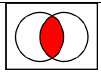
\includegraphics[scale=1]{Intersection}
\end{minipage}
\end{theo}



\begin{theo}[Difference] 
\begin{minipage}{0.7\linewidth}
\begin{itemize}
\item Means "What does A have which B does not"
\item Written as $A - B$ 
\item Can also be written as $A \setminus B $
\item SQL: \\\code{SELECT A, B \\ FROM SetA \\INNER JOIN SetB \\ON A.a = b.a}
\end{itemize}
\end{minipage}
\hspace{0.25cm}
\begin{minipage}{0.25\linewidth}
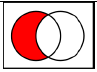
\includegraphics[scale=1]{Difference}
\end{minipage}

\end{theo}



\newpage
\section{Logic}
\begin{minipage}[t]{0.65\linewidth}
\begin{theo}[Basic] 
\begin{itemize}
\item True or false
\item Truth table
\item \textbf{Open sentence} -- 1 or more variables, $x,y$ in a \textbf{domain}
\item \textbf{Open sentence over the domain} -- $P(x)$
\begin{itemize}
\item $P(x): x+1 \geq 1$ is over the domain $\mathbb{Z}$ (integers)
\end{itemize}
\item \textbf{Negation} -- means "not"
\end{itemize}
\end{theo}
\end{minipage}
\hspace{0.10cm}
\begin{minipage}[t]{0.3\linewidth}
\begin{itemize}
\item[] \underline{Disposition}
\item Basic
\item Dis- and con-junction: $\vee, \wedge$
\item Implies and biconditional: $\Rightarrow \& \Leftrightarrow$
\item Logical equivalence: $\equiv$
\item De Morgan's laws
\item Quantifiers: $\forall, \exists$
\end{itemize}
\end{minipage}

\begin{theo}[Disjunctions and conjunctions] 
\begin{itemize}
\item \textbf{Disjunction} -- "or", written as $P \vee Q$. \textit{Any of them true?}
\begin{itemize}
\item \textbf{Exclusive or} -- xor
\end{itemize}
\item \textbf{Conjunction} -- "and", written as $P\wedge Q$. "Are both true?"
\end{itemize}
\end{theo}

\begin{theo}[Implies and biconditional]

\begin{minipage}{0.6\linewidth} 
\begin{itemize}
\item $P \Rightarrow Q$ -- politician logic.
\item $P$ is also called a \textbf{hypothesis / premesis}
\item $Q$ is the \textbf{conclusion}
\item $Q \Rightarrow P$ is a \textbf{converse}
\item \textbf{Biconditional}, written as $P \Leftrightarrow Q$ and said "$P$ is equivalent to $Q$" or "If and only if"
\end{itemize}
\end{minipage}
\hspace{0.1cm}
\begin{minipage}{0.3\linewidth}

\begin{tabular}{cc|c}
P & Q & $P \Rightarrow Q)$\\ 
\hline
T & T & T \\ 
T & F & F \\
F & T & T \\
F & F & T
\end{tabular} 
\end{minipage}
\end{theo}

\begin{theo}[Logical equivalence and  fundamental properties] 
\begin{itemize}
\item $ P \vee Q \equiv Q \vee P$ (Commutative law)
\item $P \vee (Q \vee R) \equiv (P \vee Q \vee R)$ (Associative law)
\item $P\vee (Q \wedge R) \equiv (P \vee Q) \wedge (P \vee R) $ (Distributive law)
\end{itemize}
\end{theo}

\begin{theo}[De Morgan's laws] 
\begin{minipage}{0.5\linewidth}
\begin{itemize}
\item Proof by truth table
\item $\neg (P \vee Q) \equiv (\neg P) \wedge (\neg Q)$
\item $\neg (P \wedge Q) \equiv (\neg P) \vee (\neg Q)$
\end{itemize}

\end{minipage}
\hspace{0.1cm}
\begin{minipage}{0.3\linewidth}

\begin{tabular}{cc|c|c}
P & Q & $\neg (P \wedge Q)$ & $(\neg P) \vee (\neg Q)$\\ 
\hline
T & T & F & F\\ 
T & F & T & T\\
F & T & T & T\\
F & F & T & T
\end{tabular} 
\end{minipage}
\end{theo}

\begin{theo}[Quantifiers] 
\begin{itemize}
\item \textbf{Universal quantifier} -- $\forall$ -- $\forall x \in \mathbb{N}, x \geq 0$
\item \textbf{Existential quantifier} -- $\exists$ -- $\exists x \in \mathbb{N}, x < 2$
\item Can be written as:  $\exists x \in \mathbb{Z}, P(x)$, where $P(x): x^2 < 1$
\end{itemize}
\end{theo}

\newpage
\section{Proofs techniques}


\begin{minipage}[t]{0.7\linewidth}
\begin{theo}[Basic] 
\begin{itemize}
\item \textbf{Axiom} -- statement whose truth is accepted without proof.
\item \textbf{Theorem} -- statement which can be verified.
\item \textbf{Corollary} -- a consequence of some earlier result and to be deduced from.
\item \textbf{Lemma} --a result used as help for another statement.
\end{itemize}
\end{theo}
\end{minipage}
\hspace{0.1cm}
\begin{minipage}[t]{0.27\linewidth}
\begin{itemize}
\item[] \underline{Disposition}
\item Basic
\item Conjecture
\item Trivial proof
\item Vacuous proof
\item Direct proof
\item Indirect / contrapositive
\item Proof by cases
\end{itemize}
\end{minipage}



\begin{theo}[Conjecture] 

\begin{minipage}[t]{0.48\linewidth}
\begin{itemize}
\item A conjecture is something we \textbf{believe to be true}, normally based on examples.
\end{itemize}
\end{minipage}
\hspace{0.1cm}
\begin{minipage}[t]{0.48\linewidth}
$1=1, \\
1+2=3, \\
1+2+3=6$.
\\
Conjecture: $1+\ldots+n=\sum\limits_{k=1}^n n= \dfrac{n(n+1)}{2}$
\end{minipage}
\end{theo}

\noindent{
\begin{minipage}[t]{0.5\linewidth}
	\begin{theo}[Trivial proof] 
		\begin{itemize}
		\item Something that is true -- no need to prove it.
		\item Let $n \in \mathbb{Z}$. If $n^3 > 0$ then 3 is odd
		\end{itemize}
	\end{theo}
\end{minipage}
\hspace{0.1cm}
\begin{minipage}[t]{0.48\linewidth}
	\begin{theo}[Vacuous proof] 
		\begin{itemize}
		\item If something is always proven wrong:
		\item Let $n \in \mathbb{Z}$. If \textbf{3 is even}, then $n^3 > 0$
		\item[] Clearly wrong!
		\end{itemize}
	\end{theo}
\end{minipage}
}


\begin{theo}[Direct proof] 
\begin{minipage}{0.75\linewidth}
\begin{itemize}
\item Show only what needs to be shown
\item $\forall x \in S, P(x) \Rightarrow Q(x)$
\item[] Show only that this is true also when $Q$ is false.
\item Is shown from lemmas and other proofs.
\end{itemize}
\end{minipage}
\hspace{0.1cm}
\begin{minipage}{0.2\linewidth}
Politician statement
\begin{tabular}{cc|c}
P & Q & P $\Rightarrow$ Q\\ 
\hline
T & T & T \\ 
T & F & F\\
F & T & T\\
F & F & T
\end{tabular} 

\end{minipage}
\end{theo}



\begin{theo}[Indirect proof / proof by contrapositive] 
\begin{minipage}{0.75\linewidth}
\begin{itemize}
\item Reverse the result and means.
\item Let $x \in S$. If $Q(x)$, then $P(x) \Rightarrow$
\item[] Let $x \in S$. If $\neg Q(x)$, then $\neg P(x)$
\end{itemize}
\end{minipage}
\hspace{0.1cm}
\begin{minipage}{0.2\linewidth}
Politician statement
\begin{tabular}{cc|c}
P & Q & $\neg P \Rightarrow \neg Q$\\ 
\hline
T & T & T \\ 
T & F & F\\
F & T & T\\
F & F & T
\end{tabular} 

\end{minipage}
\end{theo}



\begin{theo}[Proof by cases] 
\begin{itemize}
\item Do subcases and show they span the result.
\item Case 1: $n$ is even (U). Case 2: $n$ is odd (L). $\mathbb{Z} = U \cup L $
\item Case 1: $n\geq0$ (U). Case 2: $n<0$ (L). $\mathbb{Z} = U \cup L$
\end{itemize}
\end{theo}


\begin{theo}[Contradiction] 
 $P \Rightarrow \neg Q$\\
"Assume there's no smallest number" -- flip it:\\
"Assume there's a smallest number called $r$ -- what about $0 < \dfrac{r}{2} < r$"
\end{theo}


\begin{theo}[Induction] 
\begin{itemize}
\item Base case $P(1)$, assuming $P(k)$ sticks
\item Induction, $P(k+1)$
\end{itemize}
\end{theo}


\begin{theo}[Counter example] 
$P(k) \not \Rightarrow Q$\\
$\forall x \in \mathbb{N}, n > 2 \rightarrow n= 1 \not > 2$
\end{theo}



\newpage
\section{Direct and contrapositive proof  techniques}

\begin{minipage}[t]{0.7\linewidth}
\begin{theo}[Basic] 
\begin{itemize}
\item \textbf{Axiom} -- statement whose truth is accepted without proof.
\item \textbf{Theorem} -- statement which can be verified.
\item \textbf{Corollary} -- a consequence of some earlier result and to be deduced from.
\item \textbf{Lemma} --a result used as help for another statement.
\end{itemize}
\end{theo}
\end{minipage}
\hspace{0.1cm}
\begin{minipage}[t]{0.25\linewidth}
\begin{itemize}
\item[] \underline{Disposition}
\item Basic
\item Deduction
\item Direct proof
\item Counter example
\end{itemize}
\end{minipage}


\begin{theo}[Direct proof] 
\begin{minipage}{0.75\linewidth}
\begin{itemize}
\item Show only what needs to be shown
\item $\forall x \in S, P(x) \Rightarrow Q(x)$
\item[] Show only that this is true also when $Q$ is false.
\item Is shown from lemmas and other proofs.
\end{itemize}
\end{minipage}
\hspace{0.1cm}
\begin{minipage}{0.2\linewidth}
Politician statement
\begin{tabular}{cc|c}
P & Q & P $\Rightarrow$ Q\\ 
\hline
T & T & T \\ 
T & F & F\\
F & T & T\\
F & F & T
\end{tabular} 

\end{minipage}
\end{theo}



\begin{theo}[Deduction]  
- given P show Q
\begin{itemize}
\item Direct proof $P \Rightarrow Q$
\item Proof by cases $P(1) \Rightarrow Q, P(2) \Rightarrow Q$
\item Proof by contrapositive $\neg Q \Rightarrow \neg P$
\end{itemize}
\end{theo}


\begin{theo}[Indirect proof / proof by contrapositive] 
\begin{minipage}{0.75\linewidth}
\begin{itemize}
\item Reverse the result and means.
\item Let $x \in S$. If $Q(x)$, then $P(x) \Rightarrow$
\item[] Let $x \in S$. If $\neg Q(x)$, then $\neg P(x)$
\end{itemize}
\end{minipage}
\hspace{0.1cm}
\begin{minipage}{0.2\linewidth}
Politician statement
\begin{tabular}{cc|c}
P & Q & $\neg P \Rightarrow \neg Q$\\ 
\hline
T & T & T \\ 
T & F & F\\
F & T & T\\
F & F & T
\end{tabular} 

\end{minipage}
\end{theo}

\subsection{Her mangler}



\newpage
\section{Counterexamples and contradictive proof techniques}

\begin{minipage}{0.7\linewidth}
\begin{theo}[Counterexample] 
\begin{itemize}
\item A counterexample is \textbf{one case} that proves a statement \textbf{wrong}
\item Example
\\
$\forall x \in \mathbb{N}, x < x^2$ \\
$x=1 \Leftrightarrow 1 < 1^2 \Leftrightarrow 1 \not < 1$
\end{itemize}
\end{theo}
\end{minipage}
\hspace{0.1cm}
\begin{minipage}{0.25\linewidth}
\begin{itemize}
\item[] \underline{Disposition} 
\item Counterexample
\item Contradiction
\item Existence proof
\item Existence disproof
\end{itemize}
\end{minipage}

\begin{theo}[Proof by contradiction] 
\begin{itemize}
\item A contradiction,$\neg Q$, is assumed to be false so that \textit{Q} is true.
\item[] $(P \Rightarrow Q) = true$ becomes $(P \Rightarrow \neg Q) = false$
\item[] $(P \Rightarrow Q) \Leftrightarrow (\neg Q \Rightarrow \neg P)$
\item Example:
\item[] Let $x, y \in \mathbb{R}^{+}$. Use a proof by contradiction to prove that if $x<y$ then $\sqrt{x} < \sqrt{y}$
\\
\\
Lets rewrite the statement:
\begin{align}
\forall x, y \in \mathbb{R}^+, &P \Rightarrow Q & P = x < y \text{ and } Q = \sqrt{x}<\sqrt{y} \\
\exists x, y \in \mathbb{R}^+, &P \Rightarrow \neg Q \\
\neg Q &= \neg(\sqrt{x} < \sqrt{y})\\
\neg\sqrt{x} &< \neg \sqrt{y} \\
\sqrt{x} &\geq \sqrt{y} & \text{Remove negation}\\
x &\geq y & \text{Square both sides}
\end{align}

Since $x<y$ and $x\geq y$ is clearly not the same, the statement is proven.
\end{itemize}
\end{theo}


\begin{theo}[Existence proofs] 
 There are two kinds:
\begin{itemize}
\item \textbf{Witness}: A single example
\item[] Example: $\exists x \in \mathbb{R}, x > 0$ and pick $x=1$
\item \textbf{General/abstract}: 
\item[] Example: $\exists p \in \text{room}, \forall p' \in \text{room}, \text{Hairlenght}(p) \geq \text{Hairlenght}(p')$
\item[] Someone in the room has longer or equal long hair than everyone else -- remember more than 1 in room.
\end{itemize}
\end{theo}


\begin{theo}[Existence Disproofs] 
\begin{itemize}
\item Just like a contradiction, but for existential it's a property that never holds:
\item $\neg \big(\exists x \in S, R(x)\big) \equiv \forall x \in S, \neg R(x)$
\end{itemize}
\end{theo}



\newpage
\section{Induction proof techniques}


\begin{minipage}{0.70\linewidth}
\begin{theo}[Well-ordered] 
\begin{itemize}
\item Nonempty subset with a least element
\begin{itemize}
\item The smallest element in a subset of a set.
\item If all numbers in the set can be listed, you can find a least element
\item If you do not have, $x \in \mathbb{Q}, x < 0$ can have a subset $(0, 10]$ and that has no listed minimum.

\end{itemize}
\end{itemize}
\end{theo}
\end{minipage}
\hspace{0.1cm}
\begin{minipage}{0.25\linewidth}
\begin{itemize}
\item[] \underline{Disposition}
\item Well-ordered
\item Basic
\item Induction hypothesis
\item Strong induction
\item Minimum counterexample
\end{itemize}
\end{minipage}



\begin{theo}[Basic] 
\begin{itemize}
\item Proves a statement $P(n)$ holds for $P(n+1)$.
\item Make \textbf{base step}: $p(1)$ is true
\item[] This is also called \textbf{the induction hypothesis}.
\item Make \textbf{induction step}: $\forall k \in \mathbb{N}, P(k) \Rightarrow P(k+1)$ is true.
\item Make conclusion: $P(n)$ is true for all natural numbers, $n$.
\end{itemize}
\end{theo}


\begin{theo}[Induction hypothesis] 
\begin{itemize}
\item Induction step is $P(k) \Rightarrow P(k+1)$
\item Remember to depend on $P(k)$
\item Without this -- no induction
\begin{itemize}
\item $\forall n \in \mathbb{Z}^+, 2^n \geq n$ (For every nonnegative integer $n$\dots)
\item Base step: $n=0$ is true since $2^0>0$. Assume $2^k>k$ gives the same.
\item Induction Step: $2^{k+1}=k+1$. When $k=0$, we have $2^{0+1}=2 > 0+1=1$. Assume $k\geq 1$. 
\item Then $2^{k+1}=2\cdot 2^k > 2k=k+k \geq k+1$.
\end{itemize}
\end{itemize}
\end{theo}



\begin{theo}[Strong induction] 
\begin{itemize}
\item We don't have to start at 1 or natural numbers.
\item We have a base (proved elsewhere), a gap where some example should be, and a \textit{prior}, $k$ which will imply $k+1$.
\item Base set: $\forall n \in \mathbb{N}, P(n) \text{ where } n \geq 10$. This gives us $P(10)$ as base case.
\item Induction step: If $P(i)$ for every integer $i$ with $10 \leq i \leq k$, then $P(k+1)$ is true for every positive integer $k$ above or equal to 10.
	\begin{itemize}
	\item Not just $P(10)$ and $P(k)$ but also all in between:
	\item[] $P(i), P(i+1), P(i+2) \ldots$
	\end{itemize}
\item Conclusion: $P(k+1)$ is true.
\end{itemize}
\end{theo}


\begin{theo}[Minimum counterexample] 
\begin{itemize}
\item Assume a statement is false.
\item Make it a contradiction, showing it is \textbf{not} false.
\item A way of getting more information for the proof.
\end{itemize}
\end{theo}



\newpage
\section{Functions}

\begin{minipage}{0.7\linewidth}
\begin{theo}[Basic] 
\begin{itemize}
\item $f: A \rightarrow B$ -- "Function $f$ from $A$ to $B$"
\item Domain: $dom(f)$ -- Entire input
\item Codomain: $codom(f)$ -- Entire output
\item Image and map: $b=f(a)$ -- $b$ is the image and $f$ maps $a$ \textbf{into} $b$.
\item Inverse image: $b=f(a)$ -- $a$ \underline{can} be the output, but not necessarily.
\item Range: $range(f)$ -- What is output (not all)
\item Onto: $range(f) = codom(f)$
\item One-to-one: Every element n the target is only hit once
\end{itemize}
\end{theo}
\end{minipage}
\hspace{0.1cm}
\begin{minipage}{0.25\linewidth}
\begin{itemize}
\item \underline{Disposition}
\item Basic
\item Onto and one-to-one
\item Identity function
\item Composition
\item Inverse function
\end{itemize}
\end{minipage}


\begin{theo}[Onto and one-to-one] 
\begin{itemize}
\item Onto or \textbf{surjective}: Multiple $f(x)$ gives $f(y)$
\item One-one or \textbf{injective}: Straight over.
\item One-one is also called \textbf{bijective} or \textbf{one-to-one correspondence} if it is both one-to-one \textit{and} onto (If range and codomain is equal)
\end{itemize}
\end{theo}


\begin{theo}[Identity function] 
\begin{itemize}
\item If $R$ is equivalence relation it's,  reflective, symmetric and transitive
\item If the function is $A \rightarrow A$ it's called \textbf{Identity}.
\item this means $R: \{ (a,a),(b,b), (c,c)\ldots\}$
\begin{itemize}
\item This is only used \textit{once} on each side
\end{itemize}
\end{itemize}
\end{theo}


\begin{theo}[Composition] 
\begin{itemize}
\item $A \rightarrow f \rightarrow B \rightarrow g \rightarrow C$
\item $(g \circ f)(x): A \rightarrow C$
\item $(g \circ f)(x) = g\big(f(x)\big) \forall a \in A$
\end{itemize}
\end{theo}


\begin{theo}[Inverse function]
\begin{itemize}
\item A set with pairs where the pairs are inverted.
\item $R = \{(a,1), (b,2)\}\\
	R^{-1}=\{(1,a),(2,b)\}$
\item $R^{-1}=\{ (b,a):(a,b) \in R\}$
\end{itemize}
\end{theo}



\newpage
\section{Relations}


\begin{minipage}{0.7\linewidth}
\begin{theo}[Basic] 
\begin{itemize}
\item $R$ is a \textbf{relation} from $A$ to $B$: $R \subseteq A \times B$
\begin{itemize}
\item $A=\{x,y,z\}, B=\{1,2\}$
\item[] $R=\{(x,2),(y,1), (y,2) \}$
\end{itemize}
\item If $(a,b) \in R$ then $a$ is \textbf{related} to $b$
\item \textbf{Domain}: $R$ -- $dom(R)$ is the subset of $A$
\begin{itemize}
\item $dom(R)=\{a \in A: (a,b) \in R \text{ for some } b \in B\}$
\end{itemize}
\item \textbf{Range}: $R$ -- $range(R)$ is a subset of $B$.
\begin{itemize}
\item $range(R)=\{b \in B: (a,b) \in R \text{ for some } a \in A\}$
\end{itemize}
\item Inverse relation: $R = R^{-1}$
\begin{itemize}
\item $R^{-1} = \{(b,a):(a,b) \in R\}$
\item \textbf{Example}: $R=\{(x,2),(y,1),(y,2)\} \rightarrow R^{-1}=\{(2,x),(1,y),(2,y)\}$
\end{itemize}
\item \textbf{Relation on a set}: If $A=\{1,2\}$ then $A \times A = \{(1,1),(1,2),(2,1),(2,2)\}$
\end{itemize}
\end{theo}
\end{minipage}
\hspace{0.1cm}
\begin{minipage}{0.25\linewidth}
\begin{itemize}
\item[] \underline{Disposition}
\item Basic
\item Reflection
\item Symmetric
\item Transitive
\item Distance
\item Equivalence relation and -class
\item Congruence modulon
\end{itemize}
\end{minipage}


\begin{theo}[Reflection] 
\begin{itemize}
\item Reflection: $\forall x, a \in A: xRa \Rightarrow aRx$
\end{itemize}
\end{theo}

\begin{theo}[Symmetric] 
\begin{itemize}
\item Symmetric: $\forall x, y \in A, xRy \Rightarrow yRx$
\end{itemize}
\end{theo}

\begin{theo}[Transitive] 
\begin{itemize}
\item Transitive: $\forall x,y,z \in A, xRy \wedge yRz \Rightarrow xRz$
\begin{itemize}
\item $A=\{1\}$ is also transitive, since $(1,1)$ and $(1,1)$ you can go to $(1,1)$.
\end{itemize}
\end{itemize}
\end{theo}

\begin{theo}[Distance] 
\begin{itemize}
\item The distance between two numbers: $|a-b|$ is the numeric value.
\end{itemize}
\end{theo}

\begin{theo}[Equivalence-relation and -class] 
\begin{itemize}
\item A relation is equivalence when \textit{reflexive, symmetric and transitive} is all applied.
\item Write up $R$ and write a class as
\item[] $[a]=\{x \in A: x R a\}$
\item[] Example:  $[a]=\{a,b\}$
\item If a set has already been described, it is written:
\item[] $[b] = [a]$
\item[] $[c] = \{c\}$
\end{itemize}
\end{theo}

\begin{theo}[Congruence Modulon] 
\begin{itemize}
\item Like modulus with modifications
\item For $a,b$ where $n \geq 2$, $a$ is \textbf{congruent to} $b$ \textbf{modulo} $n$.
\item[] Example: $24 \equiv 6 (\text{mod 9})$
\item[] $\{0, 9, 18\} + 6 = 24$
\item[] Example: 
\end{itemize}
\end{theo}


\end{document}
